Le co-encadrement du stage par Rama Gottfried, qui cumule le statut de chercheur et de compositeur multimédia, a permis une réelle interaction entre informaticien et compositeur aidant à la démarche d'amélioration du logiciel \textit{symbolist}, et à la constitution de nouvelles fonctionnalités. Au-delà du développement logiciel, la conception de fonctionnalités pour \textit{symbolist} a également conduit à une réflexion sur des thématiques de recherche liées à la notation musicale.
Aussi, les aspects scientifiques qui sont discutés ci-après ont émergés lors de la définition de nouvelles \textit{user stories} pour \textit{symbolist}.

\paragraph{La partition, contrôleuse des paramètres de production sonore} Une partition peut-être vue comme une suite d'instructions (d'évènements) pour exécuter une pièce musicale \cite{bosseur2005}. Contrairement aux interactions traditionnelles où la partition est décodée par l'interprète humain pour produire de la musique, dans un environnement numérique, la partition contrôle un ou plusieurs processus informatiques (qui deviennent à leur tour des interprètes) dans le but de produire un résultat musical (ou multimédia).
Dans \textit{symbolist}, chaque symbole de la partition est décrit par un bundle OSC (voir section \ref{sec:geneseSymbolist}), qui liste, dans un format standardisé (couples adresse-valeur), les attributs du symbole associé.
Le format OSC étant standard en informatique musicale, \textit{symbolist} en tire avantage pour pouvoir communiquer des informations contenues dans une partition à d'autres processus informatiques (application, objets, composants logiciels…), dans le but de contrôler leurs paramètres d'entrées.
Alors, la question suivante se pose: comment lier, dans un paradigme de communication OSC, les attributs d'un symbole aux paramètres d'entrée d'un processus informatique?

Une exemple simple peut être pris pour illustré la nécessité de connexion entre attributs de symbole et paramètres de processus. La figure \ref{fig:linkingParameters} présente un exemple de partition créée avec \textit{symbolist} qui a pour but de contrôler la hauteur du son produit par un synthétiseur.

\begin{figure}[H]
	\centering
	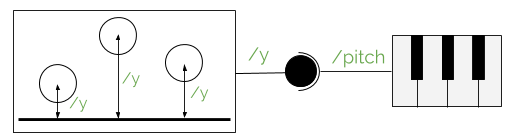
\includegraphics[keepaspectratio=true, width=\textwidth]{StructurationRecherche/i/linkingParameters.png}
	\caption{Liaison de paramètres entre une partition et un synthétiseur}
	\label{fig:linkingParameters}
	\small
	\textit{ A gauche, une partition \textit{symbolist} constitué d'un trait horizontal et d'une suite de cercles placés plus ou moins haut selon l'axe vertical. A droite, un synthétiseur, pouvant représenté un objet (au sens instance de classe), une application, ou une machine indépendante. }
\end{figure}


Dans la figure \ref{fig:linkingParameters}, le formalisme graphique utilisé pour exprimer la connexion entre les paramètres de sortie de la partition et les paramètres d'entrée du synthétiseur est celui défini par UML 2.5.1 pour modéliser les architectures de composants \cite{omg2017}. Ici, le cercle noir attaché à la partition modélise un paramètre de sortie (\textit{interface fournie}, le message OSC \texttt{/y}), et l'arc de cercle attaché au synthétiseur représente un paramètre d'entrée (\textit{interface requise}, le message OSC \texttt{/pitch}).
Dans notre exemple, le synthétiseur a besoin de l'information \texttt{/pitch}, qui représente la hauteur du son à produire en Hertz, pour pouvoir fonctionner.
De fait, connecter le paramètre \texttt{/pitch} du synthétiseur au message \texttt{/y} envoyé par la partition lie les deux valeurs selon l'expression: $/pitch = f(/y)$. Soit, la hauteur du son produit par le synthétiseur est une fonction de la hauteur des cercles sur l'axe vertical de la partition.
Lors de la lecture temporelle de la partition, le changement de hauteur des cercles va faire varier la hauteur (en Hertz) du son produit par le synthétiseur. 